\documentclass[10pt,a4paper]{article}
\usepackage[utf8]{inputenc}
\usepackage[top=2cm,bottom=2cm,left=2cm,right=2cm]{geometry}
\usepackage{amsmath}
\usepackage{amssymb}
\usepackage{tikz}
\usetikzlibrary{calc,patterns}
\usepackage[dvipsnames,svgnames]{xcolor}
\usepackage{hyperref}

% Anchor persamaan unik meski nomor di-reset per blok.
\newcounter{eqblock}
\newcommand{\reseteq}{%
  \stepcounter{eqblock}%
  \setcounter{equation}{0}%
  \renewcommand{\theHequation}{\arabic{eqblock}.\arabic{equation}}%
}

\title{Tugas Minggu 2 : Pertidaksamaan Nilai Mutlak}
\author{Matematika untuk Sistem Informasi}
\date{}

\begin{document}

\maketitle

Tentukan Himpunan Penyelesaian (HP) untuk setiap pertidaksamaan nilai mutlak berikut:

\begin{enumerate}

%===========================================================
\item $|x + 2| < 1$

\textbf{Jawab:}

\begin{itemize}
\item \textbf{Cara 1: Sifat 2, $|x| < a \iff -a < x < a$}

\begin{itemize}
\item \textbf{Langkah 1: Terapkan Sifat 2}

\reseteq
\begin{align}
|x+2| &< 1 \quad \text{(Pertidaksamaan awal)} \\
\text{Menggunakan sifat 2: } |x| &< a \Leftrightarrow -a < x < a \\
|x+2| &< 1 \Leftrightarrow -1 < x+2 < 1 \quad \text{(Sifat 2 dengan } a = 1) \\
-1 - 2 &< x+2 - 2 < 1 - 2 \quad \text{(Kurangi 2 pada semua bagian)} \\
-3 &< x < -1 \quad \text{(Solusi)}
\end{align}

\item \textbf{Langkah 2: Gambar Garis Bilangan}

\begin{center}
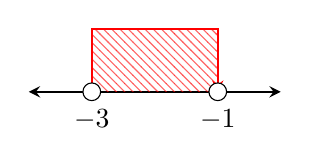
\begin{tikzpicture}[scale=0.8]

% Gambar garis bilangan utama dengan panah di kedua ujung
\draw[thick,stealth-stealth] (-4,0)--(0,0);

% Gambar garis merah untuk himpunan penyelesaian (-3 < x < -1)
\draw[thick,-stealth,Red] (-3,0)--(-3,1)--(-1,1)--(-1,0);

% Gambar arsiran untuk daerah penyelesaian
\path[pattern=north west lines,opacity=.6,pattern color=Red] (-3,0)--(-3,1)--(-1,1)--(-1,0)--cycle;

% Gambar lingkaran kosong di x = -3 dan x = -1 (karena -3 < x < -1)
\filldraw[black,fill=white] (-3,0) node[below,yshift=-.1cm] {$-3$} circle (0.4em);
\filldraw[black,fill=white] (-1,0) node[below,yshift=-.1cm] {$-1$} circle (0.4em);

\end{tikzpicture}
\end{center}

\item \textbf{Langkah 3: Tentukan HP}

$\text{HP} = (-3, -1)$

\end{itemize}

\item \textbf{Cara 2: Sifat 1, $|x| = \sqrt{x^2}$}

\begin{itemize}
\item \textbf{Langkah 1: Terapkan Sifat 1}

\reseteq
\begin{align}
|x+2| &< 1 \quad \text{(Pertidaksamaan awal)} \\
\text{Menggunakan sifat 1: } |x+2| &= \sqrt{(x+2)^2} \\
\sqrt{(x+2)^2} &< 1 \\
(\sqrt{(x+2)^2})^2 &< 1^2 \quad \text{(Kuadratkan kedua ruas)} \\
(x+2)^2 &< 1 \quad \text{(Sederhanakan)} \\
(x+2)^2 - 1 &< 1 - 1 \quad \text{(Kurangi 1 pada kedua ruas)} \\
(x+2)^2 - 1 &< 0 \quad \text{(Sederhanakan)} \\
\text{Ekspansi: } x^2 + 2 \cdot x \cdot 2 + 2^2 - 1 &< 0 \\
x^2 + 4x + 3 &< 0 \\
\text{Faktorkan: } (x + 1)(x + 3) &< 0
\end{align}

\item \textbf{Langkah 2: Tentukan Titik Kritis}

\reseteq
\begin{align}
x + 1 &= 0 \Rightarrow x = -1 \quad \text{(Pembuat nol faktor pertama)} \\
x + 3 &= 0 \Rightarrow x = -3 \quad \text{(Pembuat nol faktor kedua)}
\end{align}

\item \textbf{Langkah 3: Analisis Tanda}

Pilih nilai $x$ yang representatif untuk setiap selang:

\reseteq
\begin{align}
\text{Selang } x < -3: \quad &\text{Pilih } x = -4 \\
(x + 1)(x + 3) &= (-4 + 1)(-4 + 3) = (-3)(-1) = 3 > 0 \quad \text{(positif)} \\
\text{Selang } -3 < x < -1: \quad &\text{Pilih } x = -2 \\
(x + 1)(x + 3) &= (-2 + 1)(-2 + 3) = (-1)(1) = -1 < 0 \quad \text{(negatif)} \\
\text{Selang } x > -1: \quad &\text{Pilih } x = 0 \\
(x + 1)(x + 3) &= (0 + 1)(0 + 3) = (1)(3) = 3 > 0 \quad \text{(positif)}
\end{align}

\item \textbf{Langkah 4: Gambar Garis Bilangan}

\begin{center}
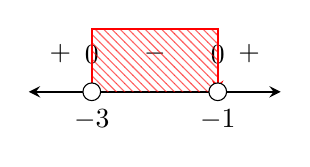
\begin{tikzpicture}[scale=0.8]

% Gambar garis bilangan utama dengan panah di kedua ujung
\draw[thick,stealth-stealth] (-4,0)--(0,0);

% Gambar tanda pada setiap selang
\node[above] at (-3.5,0.3) {$+$};
\node[above] at (-3,0.3) {$0$};
\node[above] at (-2,0.3) {$-$};
\node[above] at (-1,0.3) {$0$};
\node[above] at (-0.5,0.3) {$+$};

% Gambar garis merah untuk himpunan penyelesaian (-3 < x < -1)
\draw[thick,-stealth,Red] (-3,0)--(-3,1)--(-1,1)--(-1,0);

% Gambar arsiran untuk daerah penyelesaian
\path[pattern=north west lines,opacity=.6,pattern color=Red] (-3,0)--(-3,1)--(-1,1)--(-1,0)--cycle;

% Gambar lingkaran kosong di x = -3 dan x = -1 (karena -3 < x < -1)
\filldraw[black,fill=white] (-3,0) node[below,yshift=-.1cm] {$-3$} circle (0.4em);
\filldraw[black,fill=white] (-1,0) node[below,yshift=-.1cm] {$-1$} circle (0.4em);

\end{tikzpicture}
\end{center}

\item \textbf{Langkah 5: Tentukan HP}

$\text{HP} = (-3, -1)$

\end{itemize}
\end{itemize}

%===========================================================
\item $|2x - 1| \geq |x + 1|$

\textbf{Jawab:}

\begin{itemize}
\item \textbf{Cara 1: Sifat 4, $|x| \geq |y| \iff x^2 \geq y^2$}

\begin{itemize}
\item \textbf{Langkah 1: Terapkan Sifat 4}

\reseteq
\begin{align}
|2x-1| &\geq |x+1| \quad \text{(Pertidaksamaan awal)} \\
\text{Menggunakan sifat 4: } |x| &\geq |y| \Leftrightarrow x^2 \geq y^2 \\
|2x-1| &\geq |x+1| \Leftrightarrow (2x-1)^2 \geq (x+1)^2 \\
(2x-1)^2 - (x+1)^2 &\geq (x+1)^2 - (x+1)^2 \quad \text{(Kurangi $(x+1)^2$)} \\
(2x-1)^2 - (x+1)^2 &\geq 0 \quad \text{(Sederhanakan)} \\
\text{Menggunakan } a^2 - b^2 &= (a + b)(a - b): \\
[(2x-1) + (x+1)][(2x-1) - (x+1)] &\geq 0 \\
(2x-1 + x+1)(2x-1 - x-1) &\geq 0 \\
(3x)(x-2) &\geq 0
\end{align}

\item \textbf{Langkah 2: Tentukan Titik Kritis}

\reseteq
\begin{align}
3x &= 0 \Rightarrow x = 0 \quad \text{(Pembuat nol faktor pertama)} \\
x-2 &= 0 \Rightarrow x = 2 \quad \text{(Pembuat nol faktor kedua)}
\end{align}

\item \textbf{Langkah 3: Analisis Tanda}

Pilih nilai $x$ yang representatif untuk setiap selang:

\reseteq
\begin{align}
\text{Selang } x < 0: \quad &\text{Pilih } x = -1 \\
(3x)(x-2) &= (3(-1))(-1-2) = (-3)(-3) = 9 > 0 \quad \text{(positif)} \\
\text{Selang } 0 < x < 2: \quad &\text{Pilih } x = 1 \\
(3x)(x-2) &= (3(1))(1-2) = (3)(-1) = -3 < 0 \quad \text{(negatif)} \\
\text{Selang } x > 2: \quad &\text{Pilih } x = 3 \\
(3x)(x-2) &= (3(3))(3-2) = (9)(1) = 9 > 0 \quad \text{(positif)}
\end{align}

\item \textbf{Langkah 4: Gambar Garis Bilangan}

\begin{center}
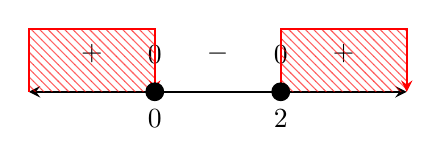
\begin{tikzpicture}[scale=0.8]

% Gambar garis bilangan utama dengan panah di kedua ujung
\draw[thick,stealth-stealth] (-2,0)--(4,0);

% Gambar tanda pada setiap selang
\node[above] at (-1,0.3) {$+$};
\node[above] at (0,0.3) {$0$};
\node[above] at (1,0.3) {$-$};
\node[above] at (2,0.3) {$0$};
\node[above] at (3,0.3) {$+$};

% Gambar garis merah untuk himpunan penyelesaian (x ≤ 0 atau x ≥ 2)
\draw[thick,-stealth,Red] (-2,0)--(-2,1)--(0,1)--(0,0);
\draw[thick,-stealth,Red] (2,0)--(2,1)--(4,1)--(4,0);

% Gambar arsiran untuk daerah penyelesaian
\path[pattern=north west lines,opacity=.6,pattern color=Red] (-2,0)--(-2,1)--(0,1)--(0,0)--cycle;
\path[pattern=north west lines,opacity=.6,pattern color=Red] (2,0)--(2,1)--(4,1)--(4,0)--cycle;

% Gambar lingkaran penuh di x = 0 dan x = 2 (karena x ≤ 0 atau x ≥ 2)
\filldraw[black,fill=black] (0,0) node[below,yshift=-.1cm] {$0$} circle (0.4em);
\filldraw[black,fill=black] (2,0) node[below,yshift=-.1cm] {$2$} circle (0.4em);

\end{tikzpicture}
\end{center}

\item \textbf{Langkah 5: Tentukan HP}

$\text{HP} = (-\infty, 0] \cup [2, \infty)$

\end{itemize}

\item \textbf{Cara 2: Sifat 1, $|x| = \sqrt{x^2}$}

\begin{itemize}
\item \textbf{Langkah 1: Terapkan Sifat 1}

\reseteq
\begin{align}
|2x-1| &\geq |x+1| \quad \text{(Pertidaksamaan awal)} \\
\text{Menggunakan sifat 1: } |2x-1| &= \sqrt{(2x-1)^2}, \quad |x+1| = \sqrt{(x+1)^2} \\
\sqrt{(2x-1)^2} &\geq \sqrt{(x+1)^2} \\
\text{Kuadratkan kedua ruas: } (\sqrt{(2x-1)^2})^2 &\geq (\sqrt{(x+1)^2})^2 \\
(2x-1)^2 &\geq (x+1)^2 \\
(2x-1)^2 - (x+1)^2 &\geq (x+1)^2 - (x+1)^2 \quad \text{(Kurangi $(x+1)^2$)} \\
(2x-1)^2 - (x+1)^2 &\geq 0 \quad \text{(Sederhanakan)} \\
\text{Menggunakan } a^2 - b^2 &= (a + b)(a - b): \\
[(2x-1) + (x+1)][(2x-1) - (x+1)] &\geq 0 \\
(2x-1 + x+1)(2x-1 - x-1) &\geq 0 \\
(3x)(x-2) &\geq 0
\end{align}

\item \textbf{Langkah 2: Tentukan Titik Kritis}

\reseteq
\begin{align}
3x &= 0 \Rightarrow x = 0 \quad \text{(Pembuat nol faktor pertama)} \\
x-2 &= 0 \Rightarrow x = 2 \quad \text{(Pembuat nol faktor kedua)}
\end{align}

\item \textbf{Langkah 3: Analisis Tanda}

Pilih nilai $x$ yang representatif untuk setiap selang:

\reseteq
\begin{align}
\text{Selang } x < 0: \quad &\text{Pilih } x = -1 \\
(3x)(x-2) &= (3(-1))(-1-2) = (-3)(-3) = 9 > 0 \quad \text{(positif)} \\
\text{Selang } 0 < x < 2: \quad &\text{Pilih } x = 1 \\
(3x)(x-2) &= (3(1))(1-2) = (3)(-1) = -3 < 0 \quad \text{(negatif)} \\
\text{Selang } x > 2: \quad &\text{Pilih } x = 3 \\
(3x)(x-2) &= (3(3))(3-2) = (9)(1) = 9 > 0 \quad \text{(positif)}
\end{align}

\item \textbf{Langkah 4: Gambar Garis Bilangan}

\begin{center}
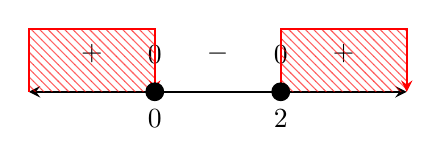
\begin{tikzpicture}[scale=0.8]

% Gambar garis bilangan utama dengan panah di kedua ujung
\draw[thick,stealth-stealth] (-2,0)--(4,0);

% Gambar tanda pada setiap selang
\node[above] at (-1,0.3) {$+$};
\node[above] at (0,0.3) {$0$};
\node[above] at (1,0.3) {$-$};
\node[above] at (2,0.3) {$0$};
\node[above] at (3,0.3) {$+$};

% Gambar garis merah untuk himpunan penyelesaian (x ≤ 0 atau x ≥ 2)
\draw[thick,-stealth,Red] (-2,0)--(-2,1)--(0,1)--(0,0);
\draw[thick,-stealth,Red] (2,0)--(2,1)--(4,1)--(4,0);

% Gambar arsiran untuk daerah penyelesaian
\path[pattern=north west lines,opacity=.6,pattern color=Red] (-2,0)--(-2,1)--(0,1)--(0,0)--cycle;
\path[pattern=north west lines,opacity=.6,pattern color=Red] (2,0)--(2,1)--(4,1)--(4,0)--cycle;

% Gambar lingkaran penuh di x = 0 dan x = 2 (karena x ≤ 0 atau x ≥ 2)
\filldraw[black,fill=black] (0,0) node[below,yshift=-.1cm] {$0$} circle (0.4em);
\filldraw[black,fill=black] (2,0) node[below,yshift=-.1cm] {$2$} circle (0.4em);

\end{tikzpicture}
\end{center}

\item \textbf{Langkah 5: Tentukan HP}

$\text{HP} = (-\infty, 0] \cup [2, \infty)$

\end{itemize}
\end{itemize}

%===========================================================
\item $\displaystyle \left|\frac{2-3x}{x+3}\right| \geq \frac{1}{4}$

\textbf{Jawab:}

Syarat penyebut: $x + 3 \neq 0$, sehingga $x \neq -3$.

\begin{itemize}
\item \textbf{Cara 1: Sifat 1, $|x| = \sqrt{x^2}$}

\begin{itemize}
\item \textbf{Langkah 1: Terapkan Sifat 1}

\reseteq
\begin{align}
\left|\frac{2-3x}{x+3}\right| &\geq \frac{1}{4} \quad \text{(Pertidaksamaan awal)} \\
\text{Menggunakan sifat 1: } \left|\frac{2-3x}{x+3}\right| &= \sqrt{\left(\frac{2-3x}{x+3}\right)^2} \\
\sqrt{\left(\frac{2-3x}{x+3}\right)^2} &\geq \frac{1}{4} \\
\text{Kuadratkan kedua ruas: } \left(\frac{2-3x}{x+3}\right)^2 &\geq \frac{1}{16} \\
\left(\frac{2-3x}{x+3}\right)^2 - \frac{1}{16} &\geq 0 \quad \text{(Kurangi $\frac{1}{16}$ pada kedua ruas)} \\
\frac{16(2-3x)^2 - (x+3)^2}{16(x+3)^2} &\geq 0 \quad \text{(Samakan penyebut)} \\
\frac{16(4-12x+9x^2) - (x^2+6x+9)}{16(x+3)^2} &\geq 0 \quad \text{(Ekspansi)} \\
\frac{64-192x+144x^2-x^2-6x-9}{16(x+3)^2} &\geq 0 \\
\frac{143x^2-198x+55}{16(x+3)^2} &\geq 0 \quad \text{(Sederhanakan)}
\end{align}

Karena $16 > 0$, tanda pecahan ditentukan oleh $\dfrac{143x^2-198x+55}{(x+3)^2}$.

\item \textbf{Langkah 2: Tentukan Titik Kritis}

Pembuat nol pembilang dan penyebut:

\reseteq
\begin{align}
143x^2 - 198x + 55 &= 0 \quad \text{(Pembuat nol pembilang)} \\
\text{Dengan } a = 143, b = -198, c = 55: & \\
x_1,x_2 &= \frac{-b \pm \sqrt{b^2 - 4ac}}{2a} \\
x_1,x_2 &= \frac{-(-198) \pm \sqrt{(-198)^2 - 4(143)(55)}}{2(143)} \\
x_1,x_2 &= \frac{198 \pm \sqrt{39204 - 31460}}{286} \\
x_1,x_2 &= \frac{198 \pm \sqrt{7744}}{286} = \frac{198 \pm 88}{286} \\
x_1 &= \frac{198 + 88}{286} = \frac{286}{286} = 1 \\
x_2 &= \frac{198 - 88}{286} = \frac{110}{286} = \frac{5}{13} \\
x + 3 &= 0 \Rightarrow x = -3 \quad \text{(Pembuat nol penyebut)}
\end{align}

\item \textbf{Langkah 3: Analisis Tanda}

Pilih nilai $x$ yang representatif untuk setiap selang:

\reseteq
\begin{align}
\text{Selang } x < -3: \quad &\text{Pilih } x = -4 \\
\frac{143x^2-198x+55}{(x+3)^2}
  &= \frac{143(-4)^2-198(-4)+55}{(-4+3)^2} \nonumber \\
  &= \frac{2288+792+55}{1} = 3135 > 0
  \quad \text{(positif)} \\
\text{Selang } -3 < x < \frac{5}{13}: \quad &\text{Pilih } x = 0 \\
\frac{143x^2-198x+55}{(x+3)^2}
  &= \frac{143(0)^2-198(0)+55}{(0+3)^2} \nonumber \\
  &= \frac{55}{9} > 0
  \quad \text{(positif)} \\
\text{Selang } \frac{5}{13} < x < 1: \quad &\text{Pilih } x = 0.5 \\
\frac{143x^2-198x+55}{(x+3)^2}
  &= \frac{143(0.5)^2-198(0.5)+55}{(0.5+3)^2} \nonumber \\
  &= \frac{35.75-99+55}{12.25} = \frac{-8.25}{12.25} < 0
  \quad \text{(negatif)} \\
\text{Selang } x > 1: \quad &\text{Pilih } x = 2 \\
\frac{143x^2-198x+55}{(x+3)^2}
  &= \frac{143(2)^2-198(2)+55}{(2+3)^2} \nonumber \\
  &= \frac{572-396+55}{25} = \frac{231}{25} > 0
  \quad \text{(positif)} \\
\text{Titik kritis:}
  &\quad x = \tfrac{5}{13},\; 1 \text{ termasuk};\; x = -3 \text{ tidak termasuk}
\end{align}

\item \textbf{Langkah 4: Gambar Garis Bilangan}

\begin{center}
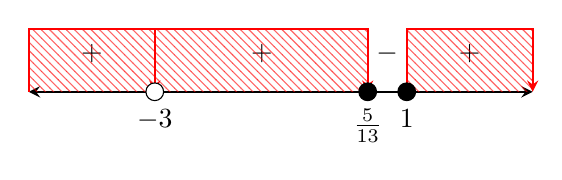
\begin{tikzpicture}[scale=0.8]

% Gambar garis bilangan utama dengan panah di kedua ujung
\draw[thick,stealth-stealth] (-5,0)--(3,0);

% Gambar tanda pada setiap selang
\node[above] at (-4,0.3) {$+$};
\node[above] at (-1.3,0.3) {$+$};
\node[above] at (0.69,0.3) {$-$};
\node[above] at (2,0.3) {$+$};

% Gambar garis merah untuk himpunan penyelesaian (x ≤ 5/13 atau x ≥ 1, x ≠ -3)
\draw[thick,-stealth,Red] (-5,0)--(-5,1)--(-3,1)--(-3,0);
\draw[thick,-stealth,Red] (-3,0)--(-3,1)--(0.38,1)--(0.38,0);
\draw[thick,-stealth,Red] (1,0)--(1,1)--(3,1)--(3,0);

% Gambar arsiran untuk daerah penyelesaian
\path[pattern=north west lines,opacity=.6,pattern color=Red] (-5,0)--(-5,1)--(-3,1)--(-3,0)--cycle;
\path[pattern=north west lines,opacity=.6,pattern color=Red] (-3,0)--(-3,1)--(0.38,1)--(0.38,0)--cycle;
\path[pattern=north west lines,opacity=.6,pattern color=Red] (1,0)--(1,1)--(3,1)--(3,0)--cycle;

% Gambar lingkaran penuh di x = 5/13 dan x = 1, lingkaran kosong di x = -3
\filldraw[black,fill=black] (0.38,0) node[below,yshift=-.1cm] {$\frac{5}{13}$} circle (0.4em);
\filldraw[black,fill=black] (1,0) node[below,yshift=-.1cm] {$1$} circle (0.4em);
\filldraw[black,fill=white] (-3,0) node[below,yshift=-.1cm] {$-3$} circle (0.4em);

\end{tikzpicture}
\end{center}

\item \textbf{Langkah 5: Tentukan HP}

$\text{HP} = (-\infty, -3) \cup \left(-3, \frac{5}{13}\right] \cup [1, \infty)$

\end{itemize}

\item \textbf{Cara 2: Sifat 5, $\left|\frac{x}{y}\right| = \frac{|x|}{|y|}$}

\begin{itemize}
\item \textbf{Langkah 1: Terapkan Sifat 5}

\reseteq
\begin{align}
\left|\frac{2-3x}{x+3}\right| &\geq \frac{1}{4} \quad \text{(Pertidaksamaan awal)} \\
\text{Menggunakan sifat 5: } \left|\frac{2-3x}{x+3}\right| &= \frac{|2-3x|}{|x+3|} \\
\frac{|2-3x|}{|x+3|} &\geq \frac{1}{4} \\
|2-3x| &\geq \frac{|x+3|}{4} \quad \text{(Kali kedua ruas dengan $|x+3| > 0$)} \\
4\,|2-3x| &\geq |x+3| \quad \text{(Kali kedua ruas dengan 4)} \\
|4|\,|2-3x| &\geq |x+3| \quad \text{($4>0$ dapat ditulis $4=|4|$)} \\
\text{Menggunakan sifat: } |ab| &= |a||b|,\quad |4||2-3x| \nonumber \\
&= |4(2-3x)| = |8-12x| \\
|8-12x| &\geq |x+3| \\
\text{Menggunakan sifat 4: } |a| \geq |b| &\Leftrightarrow a^2 \geq b^2 \\
(8-12x)^2 &\geq (x+3)^2 \\
(8-12x)^2 - (x+3)^2 &\geq 0 \quad \text{(Kurangi $(x+3)^2$ pada kedua ruas)} \\
\text{Menggunakan } a^2 - b^2 &= (a + b)(a - b): \\
[(8-12x) + (x+3)][(8-12x) - (x+3)] &\geq 0 \\
(8-12x + x+3)(8-12x - x-3) &\geq 0 \\
(11-11x)(5-13x) &\geq 0
\end{align}

\item \textbf{Langkah 2: Tentukan Titik Kritis}

\reseteq
\begin{align}
11-11x &= 0 \Rightarrow x = 1 \quad \text{(Pembuat nol faktor pertama)} \\
5-13x &= 0 \Rightarrow x = \frac{5}{13} \quad \text{(Pembuat nol faktor kedua)} \\
x+3 &= 0 \Rightarrow x = -3 \quad \text{(Syarat penyebut, } x \neq -3\text{)}
\end{align}

\item \textbf{Langkah 3: Analisis Tanda}

Pilih nilai $x$ yang representatif untuk setiap selang:

\reseteq
\begin{align}
\text{Selang } x < -3: \quad &\text{Pilih } x = -4 \\
(11-11x)(5-13x) &= (11+44)(5+52) \nonumber \\
&= (55)(57) = 3135 > 0 \quad \text{(positif)} \\
\text{Selang } -3 < x < \frac{5}{13}: \quad &\text{Pilih } x = 0 \\
(11-11x)(5-13x) &= (11)(5) = 55 > 0 \quad \text{(positif)} \\
\text{Selang } \frac{5}{13} < x < 1: \quad &\text{Pilih } x = 0.5 \\
(11-11x)(5-13x) &= (11-5.5)(5-6.5) \nonumber \\
&= (5.5)(-1.5) = -8.25 < 0 \quad \text{(negatif)} \\
\text{Selang } x > 1: \quad &\text{Pilih } x = 2 \\
(11-11x)(5-13x) &= (11-22)(5-26) \nonumber \\
&= (-11)(-21) = 231 > 0 \quad \text{(positif)}
\end{align}

\item \textbf{Langkah 4: Gambar Garis Bilangan}

\begin{center}
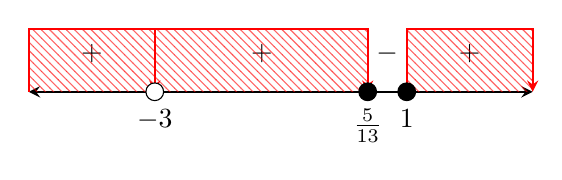
\begin{tikzpicture}[scale=0.8]

% Gambar garis bilangan utama dengan panah di kedua ujung
\draw[thick,stealth-stealth] (-5,0)--(3,0);

% Gambar tanda pada setiap selang
\node[above] at (-4,0.3) {$+$};
\node[above] at (-1.3,0.3) {$+$};
\node[above] at (0.69,0.3) {$-$};
\node[above] at (2,0.3) {$+$};

% Gambar garis merah untuk himpunan penyelesaian (x ≤ 5/13 atau x ≥ 1, x ≠ -3)
\draw[thick,-stealth,Red] (-5,0)--(-5,1)--(-3,1)--(-3,0);
\draw[thick,-stealth,Red] (-3,0)--(-3,1)--(0.38,1)--(0.38,0);
\draw[thick,-stealth,Red] (1,0)--(1,1)--(3,1)--(3,0);

% Gambar arsiran untuk daerah penyelesaian
\path[pattern=north west lines,opacity=.6,pattern color=Red] (-5,0)--(-5,1)--(-3,1)--(-3,0)--cycle;
\path[pattern=north west lines,opacity=.6,pattern color=Red] (-3,0)--(-3,1)--(0.38,1)--(0.38,0)--cycle;
\path[pattern=north west lines,opacity=.6,pattern color=Red] (1,0)--(1,1)--(3,1)--(3,0)--cycle;

% Gambar lingkaran penuh di x = 5/13 dan x = 1, lingkaran kosong di x = -3
\filldraw[black,fill=black] (0.38,0) node[below,yshift=-.1cm] {$\frac{5}{13}$} circle (0.4em);
\filldraw[black,fill=black] (1,0) node[below,yshift=-.1cm] {$1$} circle (0.4em);
\filldraw[black,fill=white] (-3,0) node[below,yshift=-.1cm] {$-3$} circle (0.4em);

\end{tikzpicture}
\end{center}

\item \textbf{Langkah 5: Tentukan HP}

$\text{HP} = (-\infty, -3) \cup \left(-3, \frac{5}{13}\right] \cup [1, \infty)$

\end{itemize}
\end{itemize}

%===========================================================
\item $\displaystyle \left|\frac{2x}{7} - 5\right| \geq 7$

\textbf{Jawab:}

\begin{itemize}
\item \textbf{Cara 1: Sifat 3, $|x| \geq a \iff x \leq -a$ atau $x \geq a$}

\begin{itemize}
\item \textbf{Langkah 1: Terapkan Sifat 3}

\reseteq
\begin{align}
\left|\frac{2x}{7}-5\right| &\geq 7 \quad \text{(Pertidaksamaan awal)} \\
\text{Menggunakan sifat 3: } |x| &\geq a \Leftrightarrow x \leq -a \text{ atau } x \geq a \\
\left|\frac{2x}{7}-5\right| &\geq 7 \Leftrightarrow \frac{2x}{7}-5 \leq -7 \text{ atau } \frac{2x}{7}-5 \geq 7
\end{align}

\item \textbf{Langkah 2: Kasus Pertama: $\frac{2x}{7}-5 \leq -7$}

\reseteq
\begin{align}
\frac{2x}{7}-5 &\leq -7 \quad \text{(Kasus pertama)} \\
\frac{2x}{7}-5 + 5 &\leq -7 + 5 \quad \text{(Tambahkan 5 pada kedua ruas)} \\
\frac{2x}{7} &\leq -2 \quad \text{(Sederhanakan)} \\
\frac{2x}{7} \cdot \frac{7}{2} &\leq -2 \cdot \frac{7}{2} \quad \text{(Kali kedua ruas dengan $\frac{7}{2}$)} \\
x &\leq -7 \quad \text{(Solusi kasus pertama)}
\end{align}

\item \textbf{Langkah 3: Kasus Kedua: $\frac{2x}{7}-5 \geq 7$}

\reseteq
\begin{align}
\frac{2x}{7}-5 &\geq 7 \quad \text{(Kasus kedua)} \\
\frac{2x}{7}-5 + 5 &\geq 7 + 5 \quad \text{(Tambahkan 5 pada kedua ruas)} \\
\frac{2x}{7} &\geq 12 \quad \text{(Sederhanakan)} \\
\frac{2x}{7} \cdot \frac{7}{2} &\geq 12 \cdot \frac{7}{2} \quad \text{(Kali kedua ruas dengan $\frac{7}{2}$)} \\
x &\geq 42 \quad \text{(Solusi kasus kedua)}
\end{align}

\item \textbf{Langkah 4: Gambar Garis Bilangan}

\begin{center}
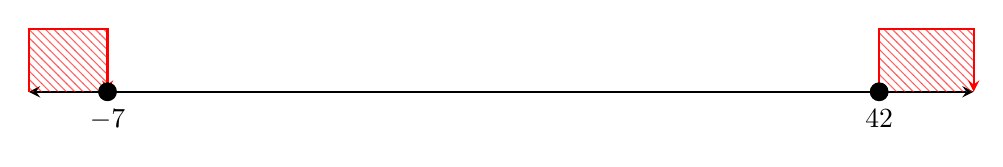
\begin{tikzpicture}[scale=0.8]

% Koordinat x digambar dengan skala 1:4 (label tetap nilai asli)
% Gambar garis bilangan utama dengan panah di kedua ujung
\draw[thick,stealth-stealth] (-3,0)--(12,0);

% Gambar garis merah untuk himpunan penyelesaian (x ≤ -7 atau x ≥ 42)
\draw[thick,-stealth,Red] (-3,0)--(-3,1)--(-1.75,1)--(-1.75,0);
\draw[thick,-stealth,Red] (10.5,0)--(10.5,1)--(12,1)--(12,0);

% Gambar arsiran untuk daerah penyelesaian
\path[pattern=north west lines,opacity=.6,pattern color=Red] (-3,0)--(-3,1)--(-1.75,1)--(-1.75,0)--cycle;
\path[pattern=north west lines,opacity=.6,pattern color=Red] (10.5,0)--(10.5,1)--(12,1)--(12,0)--cycle;

% Gambar lingkaran penuh di x = -7 dan x = 42 (karena x ≤ -7 atau x ≥ 42)
\filldraw[black,fill=black] (-1.75,0) node[below,yshift=-.1cm] {$-7$} circle (0.4em);
\filldraw[black,fill=black] (10.5,0) node[below,yshift=-.1cm] {$42$} circle (0.4em);

\end{tikzpicture}
\end{center}

\item \textbf{Langkah 5: Tentukan HP}

$\text{HP} = (-\infty, -7] \cup [42, \infty)$

\end{itemize}

\item \textbf{Cara 2: Sifat 1, $|x| = \sqrt{x^2}$}

\begin{itemize}
\item \textbf{Langkah 1: Terapkan Sifat 1}

\reseteq
\begin{align}
\left|\frac{2x}{7}-5\right| &\geq 7 \quad \text{(Pertidaksamaan awal)} \\
\text{Menggunakan sifat 1: } \left|\frac{2x}{7}-5\right| &= \sqrt{\left(\frac{2x}{7}-5\right)^2} \\
\sqrt{\left(\frac{2x}{7}-5\right)^2} &\geq 7 \\
\text{Kuadratkan kedua ruas: } \left(\frac{2x}{7}-5\right)^2 &\geq 49 \\
\left(\frac{2x}{7}-5\right)^2 - 49 &\geq 0 \quad \text{(Kurangi 49 pada kedua ruas)} \\
\text{Ekspansi: } \left(\frac{2x}{7}\right)^2 - 2 \cdot \frac{2x}{7} \cdot 5 + 5^2 - 49 &\geq 0 \\
\frac{4x^2}{49} - \frac{20x}{7} + 25 - 49 &\geq 0 \\
\frac{4x^2}{49} - \frac{20x}{7} - 24 &\geq 0 \\
\left(\frac{4x^2}{49} - \frac{20x}{7} - 24\right) \cdot 49 &\geq 0 \cdot 49 \quad \text{(Kali kedua ruas dengan 49)} \\
4x^2 - 140x - 1176 &\geq 0 \quad \text{(Sederhanakan)} \\
x^2 - 35x - 294 &\geq 0 \quad \text{(Bagi kedua ruas dengan 4)} \\
\text{Faktorkan: } (x + 7)(x - 42) &\geq 0
\end{align}

\item \textbf{Langkah 2: Tentukan Titik Kritis}

\reseteq
\begin{align}
x + 7 &= 0 \Rightarrow x = -7 \quad \text{(Pembuat nol faktor pertama)} \\
x - 42 &= 0 \Rightarrow x = 42 \quad \text{(Pembuat nol faktor kedua)}
\end{align}

\item \textbf{Langkah 3: Analisis Tanda}

Pilih nilai $x$ yang representatif untuk setiap selang:

\reseteq
\begin{align}
\text{Selang } x < -7: \quad &\text{Pilih } x = -10 \\
(x + 7)(x - 42) &= (-10 + 7)(-10 - 42) = (-3)(-52) = 156 > 0 \quad \text{(positif)} \\
\text{Selang } -7 < x < 42: \quad &\text{Pilih } x = 0 \\
(x + 7)(x - 42) &= (0 + 7)(0 - 42) = (7)(-42) = -294 < 0 \quad \text{(negatif)} \\
\text{Selang } x > 42: \quad &\text{Pilih } x = 50 \\
(x + 7)(x - 42) &= (50 + 7)(50 - 42) = (57)(8) = 456 > 0 \quad \text{(positif)}
\end{align}

\item \textbf{Langkah 4: Gambar Garis Bilangan}

\begin{center}
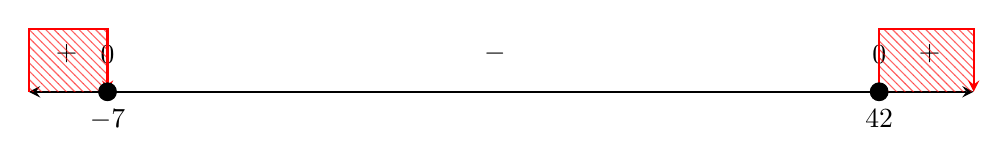
\begin{tikzpicture}[scale=0.8]

% Koordinat x digambar dengan skala 1:4 (label tetap nilai asli)
% Gambar garis bilangan utama dengan panah di kedua ujung
\draw[thick,stealth-stealth] (-3,0)--(12,0);

% Gambar tanda pada setiap selang
\node[above] at (-2.4,0.3) {$+$};
\node[above] at (-1.75,0.3) {$0$};
\node[above] at (4.4,0.3) {$-$};
\node[above] at (10.5,0.3) {$0$};
\node[above] at (11.3,0.3) {$+$};

% Gambar garis merah untuk himpunan penyelesaian (x ≤ -7 atau x ≥ 42)
\draw[thick,-stealth,Red] (-3,0)--(-3,1)--(-1.75,1)--(-1.75,0);
\draw[thick,-stealth,Red] (10.5,0)--(10.5,1)--(12,1)--(12,0);

% Gambar arsiran untuk daerah penyelesaian
\path[pattern=north west lines,opacity=.6,pattern color=Red] (-3,0)--(-3,1)--(-1.75,1)--(-1.75,0)--cycle;
\path[pattern=north west lines,opacity=.6,pattern color=Red] (10.5,0)--(10.5,1)--(12,1)--(12,0)--cycle;

% Gambar lingkaran penuh di x = -7 dan x = 42 (karena x ≤ -7 atau x ≥ 42)
\filldraw[black,fill=black] (-1.75,0) node[below,yshift=-.1cm] {$-7$} circle (0.4em);
\filldraw[black,fill=black] (10.5,0) node[below,yshift=-.1cm] {$42$} circle (0.4em);

\end{tikzpicture}
\end{center}

\item \textbf{Langkah 5: Tentukan HP}

$\text{HP} = (-\infty, -7] \cup [42, \infty)$

\end{itemize}
\end{itemize}

%===========================================================
\item $\displaystyle \left|\frac{x-1}{3x+1}\right| \leq \frac{7}{2}$

\textbf{Jawab:}

Syarat penyebut: $3x + 1 \neq 0$, sehingga $x \neq -\frac{1}{3}$.

\begin{itemize}
\item \textbf{Cara 1: Sifat 2, $|x| \leq a \iff -a \leq x \leq a$}

\begin{itemize}
\item \textbf{Langkah 1: Terapkan Sifat 2}

\reseteq
\begin{align}
\left|\frac{x-1}{3x+1}\right| &\leq \frac{7}{2} \quad \text{(Pertidaksamaan awal)} \\
\text{Menggunakan sifat 2: } |x| &\leq a \Leftrightarrow -a \leq x \leq a \\
\left|\frac{x-1}{3x+1}\right| &\leq \frac{7}{2} \Leftrightarrow -\frac{7}{2} \leq \frac{x-1}{3x+1} \leq \frac{7}{2}
\end{align}

Pertidaksamaan ganda ini dipecah menjadi dua kasus yang harus dipenuhi bersamaan:
\[
\frac{x-1}{3x+1} \geq -\frac{7}{2} \quad \text{dan} \quad \frac{x-1}{3x+1} \leq \frac{7}{2}.
\]

\item \textbf{Langkah 2: Kasus Pertama: $\frac{x-1}{3x+1} \geq -\frac{7}{2}$}

\reseteq
\begin{align}
\frac{x-1}{3x+1} + \frac{7}{2} &\geq 0 \quad \text{(Tambahkan $\frac{7}{2}$ pada kedua ruas)} \\
\frac{2(x-1) + 7(3x+1)}{2(3x+1)} &\geq 0 \quad \text{(Samakan penyebut)} \\
\frac{2x-2 + 21x+7}{2(3x+1)} &\geq 0 \\
\frac{23x+5}{2(3x+1)} &\geq 0 \\
\frac{23x+5}{3x+1} &\geq 0 \quad \text{(Kali kedua ruas dengan 2)}
\end{align}

Titik kritis: $23x + 5 = 0 \Rightarrow x = -\frac{5}{23}$ (pembilang) dan $3x + 1 = 0 \Rightarrow x = -\frac{1}{3}$ (penyebut).
Urutannya $-\frac{1}{3} < -\frac{5}{23}$.

\reseteq
\begin{align}
\text{Selang } x < -\frac{1}{3}: \quad &\text{Pilih } x = -1 \\
\frac{23x+5}{3x+1} &= \frac{-23+5}{-3+1} = \frac{-18}{-2} = 9 > 0 \quad \text{(positif)} \\
\text{Selang } -\frac{1}{3} < x < -\frac{5}{23}: \quad &\text{Pilih } x = -0.3 \\
\frac{23x+5}{3x+1} &= \frac{-6.9+5}{-0.9+1} = \frac{-1.9}{0.1} = -19 < 0 \quad \text{(negatif)} \\
\text{Selang } x > -\frac{5}{23}: \quad &\text{Pilih } x = 0 \\
\frac{23x+5}{3x+1} &= \frac{5}{1} = 5 > 0 \quad \text{(positif)}
\end{align}

Solusi kasus pertama: $x < -\frac{1}{3}$ atau $x \geq -\frac{5}{23}$.

\item \textbf{Langkah 3: Kasus Kedua: $\frac{x-1}{3x+1} \leq \frac{7}{2}$}

\reseteq
\begin{align}
\frac{x-1}{3x+1} - \frac{7}{2} &\leq 0 \quad \text{(Kurangi $\frac{7}{2}$ pada kedua ruas)} \\
\frac{2(x-1) - 7(3x+1)}{2(3x+1)} &\leq 0 \quad \text{(Samakan penyebut)} \\
\frac{2x-2 - 21x-7}{2(3x+1)} &\leq 0 \\
\frac{-19x-9}{2(3x+1)} &\leq 0 \\
\frac{-19x-9}{3x+1} &\leq 0 \quad \text{(Kali kedua ruas dengan 2)} \\
\frac{19x+9}{3x+1} &\geq 0 \quad \text{(Kali kedua ruas dengan $-1$, tanda berubah)}
\end{align}

Titik kritis: $19x + 9 = 0 \Rightarrow x = -\frac{9}{19}$ (pembilang) dan $x = -\frac{1}{3}$ (penyebut).
Urutannya $-\frac{9}{19} < -\frac{1}{3}$.

\reseteq
\begin{align}
\text{Selang } x < -\frac{9}{19}: \quad &\text{Pilih } x = -1 \\
\frac{19x+9}{3x+1} &= \frac{-19+9}{-3+1} = \frac{-10}{-2} = 5 > 0 \quad \text{(positif)} \\
\text{Selang } -\frac{9}{19} < x < -\frac{1}{3}: \quad &\text{Pilih } x = -0.4 \\
\frac{19x+9}{3x+1} &= \frac{-7.6+9}{-1.2+1} = \frac{1.4}{-0.2} = -7 < 0 \quad \text{(negatif)} \\
\text{Selang } x > -\frac{1}{3}: \quad &\text{Pilih } x = 0 \\
\frac{19x+9}{3x+1} &= \frac{9}{1} = 9 > 0 \quad \text{(positif)}
\end{align}

Solusi kasus kedua: $x \leq -\frac{9}{19}$ atau $x > -\frac{1}{3}$.

\item \textbf{Langkah 4: Gambar Garis Bilangan dan Irisan}

Urutan titik kritis: $-\frac{9}{19} < -\frac{1}{3} < -\frac{5}{23}$.

\begin{itemize}
\item Gambar Garis Bilangan untuk kasus pertama: $x < -\frac{1}{3}$ atau $x \geq -\frac{5}{23}$
\begin{center}
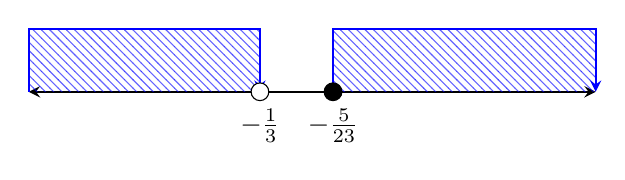
\begin{tikzpicture}[scale=0.8]

% Koordinat x digambar dengan skala 10:1 (label tetap nilai asli)
% Gambar garis bilangan utama dengan panah di kedua ujung
\draw[thick,stealth-stealth] (-7,0)--(2,0);

% Gambar garis biru untuk kasus pertama
\draw[thick,-stealth,Blue] (-7,0)--(-7,1)--(-3.33,1)--(-3.33,0);
\draw[thick,-stealth,Blue] (-2.17,0)--(-2.17,1)--(2,1)--(2,0);

% Gambar arsiran untuk daerah penyelesaian kasus pertama
\path[pattern=north west lines,opacity=.6,pattern color=Blue] (-7,0)--(-7,1)--(-3.33,1)--(-3.33,0)--cycle;
\path[pattern=north west lines,opacity=.6,pattern color=Blue] (-2.17,0)--(-2.17,1)--(2,1)--(2,0)--cycle;

% Lingkaran kosong di x = -1/3 (penyebut nol), lingkaran penuh di x = -5/23
\filldraw[black,fill=white] (-3.33,0) node[below,yshift=-.1cm] {$-\frac{1}{3}$} circle (0.4em);
\filldraw[black,fill=black] (-2.17,0) node[below,yshift=-.1cm] {$-\frac{5}{23}$} circle (0.4em);

\end{tikzpicture}
\end{center}

\item Gambar Garis Bilangan untuk kasus kedua: $x \leq -\frac{9}{19}$ atau $x > -\frac{1}{3}$
\begin{center}
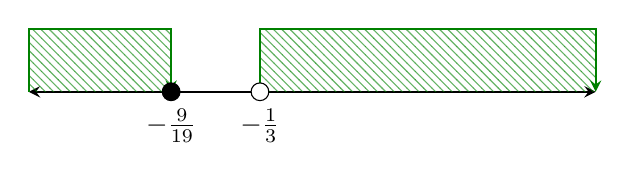
\begin{tikzpicture}[scale=0.8]

% Koordinat x digambar dengan skala 10:1 (label tetap nilai asli)
% Gambar garis bilangan utama dengan panah di kedua ujung
\draw[thick,stealth-stealth] (-7,0)--(2,0);

% Gambar garis hijau untuk kasus kedua
\draw[thick,-stealth,Green] (-7,0)--(-7,1)--(-4.74,1)--(-4.74,0);
\draw[thick,-stealth,Green] (-3.33,0)--(-3.33,1)--(2,1)--(2,0);

% Gambar arsiran untuk daerah penyelesaian kasus kedua
\path[pattern=north west lines,opacity=.6,pattern color=Green] (-7,0)--(-7,1)--(-4.74,1)--(-4.74,0)--cycle;
\path[pattern=north west lines,opacity=.6,pattern color=Green] (-3.33,0)--(-3.33,1)--(2,1)--(2,0)--cycle;

% Lingkaran penuh di x = -9/19, lingkaran kosong di x = -1/3 (penyebut nol)
\filldraw[black,fill=black] (-4.74,0) node[below,yshift=-.1cm] {$-\frac{9}{19}$} circle (0.4em);
\filldraw[black,fill=white] (-3.33,0) node[below,yshift=-.1cm] {$-\frac{1}{3}$} circle (0.4em);

\end{tikzpicture}
\end{center}

\item Gambar Garis Bilangan untuk irisan kedua kasus: $x \leq -\frac{9}{19}$ atau $x \geq -\frac{5}{23}$
\begin{center}
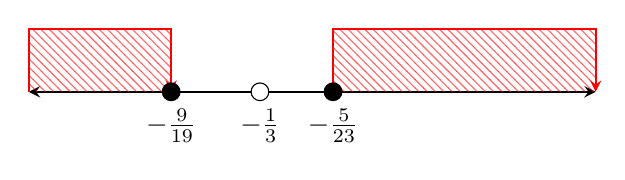
\begin{tikzpicture}[scale=0.8]

% Koordinat x digambar dengan skala 10:1 (label tetap nilai asli)
% Gambar garis bilangan utama dengan panah di kedua ujung
\draw[thick,stealth-stealth] (-7,0)--(2,0);

% Gambar garis merah untuk himpunan penyelesaian (x ≤ -9/19 atau x ≥ -5/23)
\draw[thick,-stealth,Red] (-7,0)--(-7,1)--(-4.74,1)--(-4.74,0);
\draw[thick,-stealth,Red] (-2.17,0)--(-2.17,1)--(2,1)--(2,0);

% Gambar arsiran untuk daerah penyelesaian
\path[pattern=north west lines,opacity=.6,pattern color=Red] (-7,0)--(-7,1)--(-4.74,1)--(-4.74,0)--cycle;
\path[pattern=north west lines,opacity=.6,pattern color=Red] (-2.17,0)--(-2.17,1)--(2,1)--(2,0)--cycle;

% Lingkaran penuh di x = -9/19 dan x = -5/23, lingkaran kosong di x = -1/3
\filldraw[black,fill=black] (-4.74,0) node[below,yshift=-.1cm] {$-\frac{9}{19}$} circle (0.4em);
\filldraw[black,fill=white] (-3.33,0) node[below,yshift=-.1cm] {$-\frac{1}{3}$} circle (0.4em);
\filldraw[black,fill=black] (-2.17,0) node[below,yshift=-.1cm] {$-\frac{5}{23}$} circle (0.4em);

\end{tikzpicture}
\end{center}
\end{itemize}

\item \textbf{Langkah 5: Tentukan HP}

$\text{HP} = \left(\left(-\infty, -\frac{1}{3}\right) \cup \left[-\frac{5}{23}, \infty\right)\right) \cap \left(\left(-\infty, -\frac{9}{19}\right] \cup \left(-\frac{1}{3}, \infty\right)\right) = \left(-\infty, -\frac{9}{19}\right] \cup \left[-\frac{5}{23}, \infty\right)$

\end{itemize}

\item \textbf{Cara 2: Sifat 5, $\left|\frac{x}{y}\right| = \frac{|x|}{|y|}$}

\begin{itemize}
\item \textbf{Langkah 1: Terapkan Sifat 5}

\reseteq
\begin{align}
\left|\frac{x-1}{3x+1}\right| &\leq \frac{7}{2} \quad \text{(Pertidaksamaan awal)} \\
\text{Menggunakan sifat 5: } \left|\frac{x-1}{3x+1}\right| &= \frac{|x-1|}{|3x+1|} \\
\frac{|x-1|}{|3x+1|} &\leq \frac{7}{2} \\
|x-1| &\leq \frac{7}{2}\,|3x+1| \quad \text{(Kali dengan $|3x+1| > 0$)} \\
2\,|x-1| &\leq 7\,|3x+1| \quad \text{(Kali kedua ruas dengan 2)} \\
|2|\,|x-1| &\leq |7|\,|3x+1| \quad \text{($2=|2|$ dan $7=|7|$)} \\
\text{Menggunakan sifat: } |ab| &= |a||b| \nonumber \\
|2x-2| &\leq |21x+7| \\
\text{Menggunakan sifat 4: } |a| \leq |b| &\Leftrightarrow a^2 \leq b^2 \\
(2x-2)^2 &\leq (21x+7)^2 \\
(2x-2)^2 - (21x+7)^2 &\leq 0 \quad \text{(Kurangi $(21x+7)^2$)} \\
\text{Menggunakan } a^2 - b^2 &= (a + b)(a - b): \\
[(2x-2) + (21x+7)][(2x-2) - (21x+7)] &\leq 0 \\
(23x+5)(-19x-9) &\leq 0 \\
-(23x+5)(19x+9) &\leq 0 \quad \text{(Keluarkan faktor negatif)} \\
(23x+5)(19x+9) &\geq 0 \quad \text{(Kali $-1$, tanda berubah)}
\end{align}

\item \textbf{Langkah 2: Tentukan Titik Kritis}

\reseteq
\begin{align}
19x+9 &= 0 \Rightarrow x = -\frac{9}{19} \quad \text{(Pembuat nol faktor pertama)} \\
23x+5 &= 0 \Rightarrow x = -\frac{5}{23} \quad \text{(Pembuat nol faktor kedua)} \\
3x+1 &= 0 \Rightarrow x = -\frac{1}{3} \quad \text{(Syarat penyebut, } x \neq -\tfrac{1}{3}\text{)}
\end{align}

Urutan titik kritis: $-\frac{9}{19} < -\frac{1}{3} < -\frac{5}{23}$.

\item \textbf{Langkah 3: Analisis Tanda}

Pilih nilai $x$ yang representatif untuk setiap selang:

\reseteq
\begin{align}
\text{Selang } x < -\frac{9}{19}: \quad &\text{Pilih } x = -1 \\
(23x+5)(19x+9) &= (-23+5)(-19+9) \nonumber \\
&= (-18)(-10) = 180 > 0 \quad \text{(positif)} \\
\text{Selang } -\frac{9}{19} < x < -\frac{5}{23}: \quad &\text{Pilih } x = -0.3 \\
(23x+5)(19x+9) &= (-6.9+5)(-5.7+9) \nonumber \\
&= (-1.9)(3.3) = -6.27 < 0 \quad \text{(negatif)} \\
\text{Selang } x > -\frac{5}{23}: \quad &\text{Pilih } x = 0 \\
(23x+5)(19x+9) &= (5)(9) = 45 > 0 \quad \text{(positif)} \\
\text{Titik kritis:}
  &\quad x = -\tfrac{9}{19},\; -\tfrac{5}{23} \text{ termasuk};\; x = -\tfrac{1}{3} \text{ tidak termasuk}
\end{align}

Titik $x = -\frac{1}{3}$ berada di selang negatif, sehingga sudah tidak termasuk HP.

\item \textbf{Langkah 4: Gambar Garis Bilangan}

\begin{center}
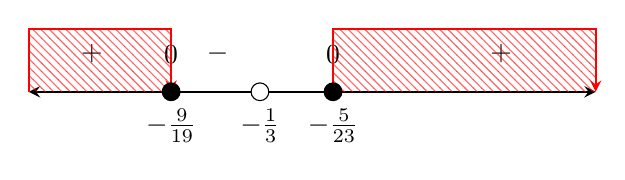
\begin{tikzpicture}[scale=0.8]

% Koordinat x digambar dengan skala 10:1 (label tetap nilai asli)
% Gambar garis bilangan utama dengan panah di kedua ujung
\draw[thick,stealth-stealth] (-7,0)--(2,0);

% Gambar tanda pada setiap selang
\node[above] at (-6,0.3) {$+$};
\node[above] at (-4.74,0.3) {$0$};
\node[above] at (-4,0.3) {$-$};
\node[above] at (-2.17,0.3) {$0$};
\node[above] at (0.5,0.3) {$+$};

% Gambar garis merah untuk himpunan penyelesaian (x ≤ -9/19 atau x ≥ -5/23)
\draw[thick,-stealth,Red] (-7,0)--(-7,1)--(-4.74,1)--(-4.74,0);
\draw[thick,-stealth,Red] (-2.17,0)--(-2.17,1)--(2,1)--(2,0);

% Gambar arsiran untuk daerah penyelesaian
\path[pattern=north west lines,opacity=.6,pattern color=Red] (-7,0)--(-7,1)--(-4.74,1)--(-4.74,0)--cycle;
\path[pattern=north west lines,opacity=.6,pattern color=Red] (-2.17,0)--(-2.17,1)--(2,1)--(2,0)--cycle;

% Lingkaran penuh di x = -9/19 dan x = -5/23, lingkaran kosong di x = -1/3
\filldraw[black,fill=black] (-4.74,0) node[below,yshift=-.1cm] {$-\frac{9}{19}$} circle (0.4em);
\filldraw[black,fill=white] (-3.33,0) node[below,yshift=-.1cm] {$-\frac{1}{3}$} circle (0.4em);
\filldraw[black,fill=black] (-2.17,0) node[below,yshift=-.1cm] {$-\frac{5}{23}$} circle (0.4em);

\end{tikzpicture}
\end{center}

\item \textbf{Langkah 5: Tentukan HP}

$\text{HP} = \left(-\infty, -\frac{9}{19}\right] \cup \left[-\frac{5}{23}, \infty\right)$

\end{itemize}
\end{itemize}

\end{enumerate}

\end{document}
